% This LaTeX was auto-generated from MATLAB code.
% To make changes, update the MATLAB code and export to LaTeX again.

\documentclass{article}

\usepackage[utf8]{inputenc}
\usepackage[T1]{fontenc}
\usepackage{lmodern}
\usepackage{graphicx}
\usepackage{color}
\usepackage{hyperref}
\usepackage{amsmath}
\usepackage{amsfonts}
\usepackage{epstopdf}
\usepackage[table]{xcolor}
\usepackage{matlab}

\sloppy
\epstopdfsetup{outdir=./}
\graphicspath{ {./neuralnet_example_images/} }

\matlabmultipletitles

\begin{document}

\matlabtitle{Implementing Neural Networks}

\begin{par}
\begin{flushleft}
We are going to tackle the problem of digit classification from image. More concretely, we are going to use the MNIST digits dataset. The explanation to load the dataset is in \href{https://lucidar.me/en/matlab/load-mnist-database-of-handwritten-digits-in-matlab/}{https://lucidar.me/en/matlab/load-mnist-database-of-handwritten-digits-in-matlab/} .
\end{flushleft}
\end{par}

\begin{matlabcode}
load ('mnist.mat')

X_train = training.images;
Y_train = training.labels;
X_test = test.images;
Y_test = test.labels;
\end{matlabcode}


\begin{matlabcode}
X_train(:,:,18)
\end{matlabcode}
\begin{matlaboutput}
ans = 28x28    
         0         0         0         0         0         0         0         0         0         0         0         0         0         0         0         0         0         0         0         0         0         0         0         0         0         0         0         0
         0         0         0         0         0         0         0         0         0         0         0         0         0         0         0         0         0         0         0         0         0         0         0         0         0         0         0         0
         0         0         0         0         0         0         0         0         0         0         0         0         0         0         0         0         0         0         0         0         0         0         0         0         0         0         0         0
         0         0         0         0         0         0         0         0         0         0         0         0         0         0         0         0         0         0         0         0         0         0         0         0         0         0         0         0
         0         0         0         0         0         0         0         0         0         0         0         0         0         0         0         0         0         0         0         0         0         0         0         0         0         0         0         0
         0         0         0         0         0         0         0         0         0         0         0         0         0         0         0         0         0         0         0    0.0431    0.7961    0.8980    0.1255         0         0         0         0         0
         0         0         0         0         0         0         0         0         0         0         0         0         0         0         0    0.1020    0.1843    0.1843    0.1176    0.3725    0.9961    0.8431    0.0510         0         0         0         0         0
         0         0         0         0         0         0         0         0         0         0         0    0.1765    0.6039    0.7255    0.7255    0.8745    0.9922    0.9922    0.5216    0.6863    1.0000    0.7373    0.0745         0         0         0         0         0
         0         0         0         0         0         0         0         0         0         0         0    0.4314    0.9922    0.9922    0.9922    0.9647    0.6314    0.8941    0.9922    0.9922    0.9961    0.3608         0         0         0         0         0         0
         0         0         0         0         0         0         0         0         0         0    0.5020    0.9608    0.9922    0.6196    0.5373    0.0824         0    0.1882    0.9137    0.9922    0.9137    0.0314         0         0         0         0         0         0

\end{matlaboutput}
\begin{matlabcode}
image (training.images(:,:,18)*255);
colormap("gray")
\end{matlabcode}
\begin{center}
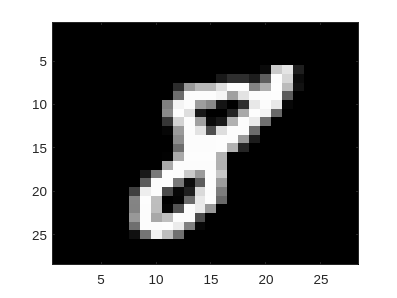
\includegraphics[width=\maxwidth{39.839438033115904em}]{figure_0.png}
\end{center}

\begin{par}
\begin{flushleft}
This images are matrices of 28x28 in grayscale. This means that our network needs a 28x28=784 sized input layer. We need to resize these matrices:
\end{flushleft}
\end{par}

\begin{matlabcode}
X_train = reshape(X_train,[784,60000])';
X_test = reshape(X_test,[784,10000])';
\end{matlabcode}


\begin{matlabcode}
Y_train(1)
\end{matlabcode}
\begin{matlaboutput}
ans = 5
\end{matlaboutput}

\begin{par}
\begin{flushleft}
The labels are expressed as the digit. We want them as a one-hot encoding.
\end{flushleft}
\end{par}

\begin{matlabcode}
TT_train = Y_train + 1; % The function ind2vec needs positive values.
TTrain = full(ind2vec(TT_train'))';
TT_test = Y_test + 1;
TTest = full(ind2vec(TT_test'))';

Y_train(18)
\end{matlabcode}
\begin{matlaboutput}
ans = 8
\end{matlaboutput}
\begin{matlabcode}
TTrain(18,:)
\end{matlabcode}
\begin{matlaboutput}
ans = 1x10    
     0     0     0     0     0     0     0     0     1     0

\end{matlaboutput}


\begin{par}
\begin{flushleft}
We can see how the 9th position of the one-hot encoded version is set to 1. This means the digit is 8.
\end{flushleft}
\end{par}

\begin{par}
\begin{flushleft}
Also, since there are 10 possible digits, we will tackle this problem as a 10-class classification, so the output layer will have 10 neurons.
\end{flushleft}
\end{par}

\begin{par}
\begin{flushleft}
For the hidden layers, we would need to decide what to do. We are going to go with one fully connected hidden layer of 32 neurons. 
\end{flushleft}
\end{par}

\begin{par}
\begin{flushleft}
We also need to initialize the weights of our network.
\end{flushleft}
\end{par}

\begin{par}
\begin{flushleft}
And the activation function and its derivative. We are using the ReLU activation function for the hidden layer, and softmax for the output layer.
\end{flushleft}
\end{par}


\begin{matlabcode}
inputLayerSize = 784;
hiddenLayer1Size = 50;
outputLayerSize = 10;
\end{matlabcode}

\begin{par}
\begin{flushleft}
We also need to initialize the weights of our network:
\end{flushleft}
\end{par}

\begin{matlabcode}
[W1,b1,Wout,bout] = generate_weights(inputLayerSize,hiddenLayer1Size,outputLayerSize,0.1);
\end{matlabcode}

\begin{par}
\begin{flushleft}
And the activation function and its derivative. We are using the sigmoid here:
\end{flushleft}
\end{par}

\begin{matlabcode}
learningRate = 0.01;
numEpochs = 20;
batchsize = 100;

accuracy_history = zeros(numEpochs, 1);

for epoch = 1:numEpochs 
    for i = 1:size(X_train, 1)/batchsize
        % Use the permuted indices to get the current example and label
        X = X_train(1+batchsize*(i-1):batchsize*i,:);
        T = TTrain(1+batchsize*(i-1):batchsize*i,:);
        
        % Feedforward
        [A1,Z1,Aout,Zout] = forward_pass(X,W1,b1,Wout,bout);
        
        % Backpropagation
        [grad_W1, grad_b1, grad_Wout, grad_bout] = backward_pass(Zout, T, Z1, X, Wout, A1);

        % Update weights and biases
        [W1, b1, Wout, bout] = update_weights(learningRate,W1,b1,Wout,bout,grad_W1,grad_b1,grad_Wout,grad_bout);
    end
    accuracy_history(epoch) = compute_accuracy(X_train, TTrain, W1, b1, Wout, bout);
    fprintf('Epoch %d: Accuracy: %0.5f\n', epoch, accuracy_history(epoch));
end
\end{matlabcode}
\begin{matlaboutput}
Epoch 1: Accuracy: 0.91012
Epoch 2: Accuracy: 0.94228
Epoch 3: Accuracy: 0.95607
Epoch 4: Accuracy: 0.96497
Epoch 5: Accuracy: 0.96605
Epoch 6: Accuracy: 0.96827
Epoch 7: Accuracy: 0.97248
Epoch 8: Accuracy: 0.97268
Epoch 9: Accuracy: 0.97395
Epoch 10: Accuracy: 0.97367
Epoch 11: Accuracy: 0.96990
Epoch 12: Accuracy: 0.97192
Epoch 13: Accuracy: 0.97407
Epoch 14: Accuracy: 0.97380
Epoch 15: Accuracy: 0.97337
Epoch 16: Accuracy: 0.97522
Epoch 17: Accuracy: 0.97515
Epoch 18: Accuracy: 0.97322
Epoch 19: Accuracy: 0.97260
Epoch 20: Accuracy: 0.97768
\end{matlaboutput}
\begin{matlabcode}

figure;
plot(1:numEpochs, accuracy_history);
title('Training Accuracy over Epochs');
xlabel('Epoch');
ylabel('Accuracy');
\end{matlabcode}
\begin{center}
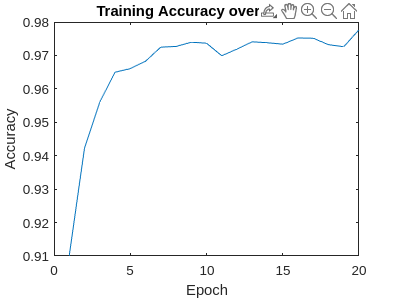
\includegraphics[width=\maxwidth{39.839438033115904em}]{figure_1.png}
\end{center}


\begin{par}
\begin{flushleft}
Test:
\end{flushleft}
\end{par}

\begin{matlabcode}
accuracy = compute_accuracy(X_test,TTest,W1,b1,Wout,bout);
fprintf('Accuracy: %0.5f\n', accuracy);
\end{matlabcode}
\begin{matlaboutput}
Accuracy: 0.95960
\end{matlaboutput}
\begin{matlabcode}

x = X_test(18,:);
pred = prediction(x,W1,b1,Wout,bout)
\end{matlabcode}
\begin{matlaboutput}
pred = 7
\end{matlaboutput}
\begin{matlabcode}
image (reshape(x*255,[28,28]));
colormap("gray")
\end{matlabcode}
\begin{center}
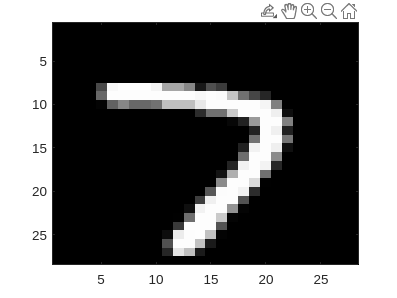
\includegraphics[width=\maxwidth{39.839438033115904em}]{figure_2.png}
\end{center}
\begin{matlabcode}

x = X_test(140,:);
pred = prediction(x,W1,b1,Wout,bout)
\end{matlabcode}
\begin{matlaboutput}
pred = 4
\end{matlaboutput}
\begin{matlabcode}
image (reshape(x*255,[28,28]));
colormap("gray")
\end{matlabcode}
\begin{center}
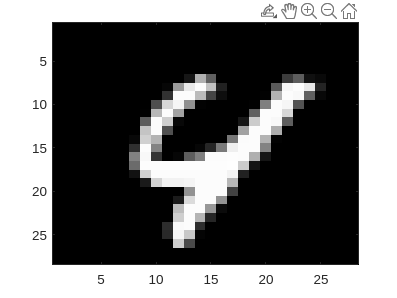
\includegraphics[width=\maxwidth{39.839438033115904em}]{figure_3.png}
\end{center}
\begin{matlabcode}

x = X_test(5442,:);
pred = prediction(x,W1,b1,Wout,bout)
\end{matlabcode}
\begin{matlaboutput}
pred = 6
\end{matlaboutput}
\begin{matlabcode}
image (reshape(x*255,[28,28]));
colormap("gray")
\end{matlabcode}
\begin{center}
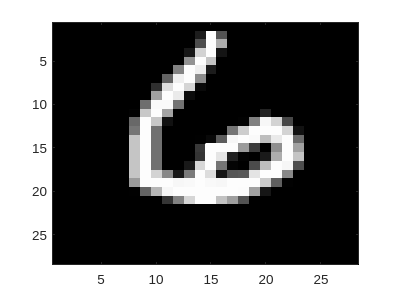
\includegraphics[width=\maxwidth{39.839438033115904em}]{figure_4.png}
\end{center}


\begin{matlabcode}
pred = -1;
real = -1;
i = 82;

while pred == real
    x = X_test(i,:);
    pred = prediction(x,W1,b1,Wout,bout);

    real = Y_test(i);

    i = i+1;
end

x = X_test(i-1,:);
pred = prediction(x,W1,b1,Wout,bout)
\end{matlabcode}
\begin{matlaboutput}
pred = 9
\end{matlaboutput}
\begin{matlabcode}
image (reshape(x*255,[28,28]));
colormap("gray")
\end{matlabcode}
\begin{center}
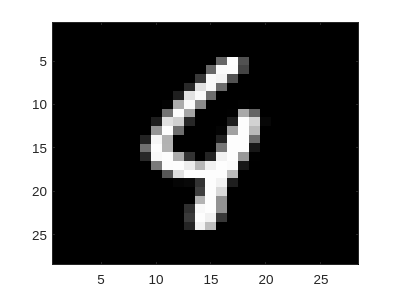
\includegraphics[width=\maxwidth{39.839438033115904em}]{figure_5.png}
\end{center}


\matlabtitle{Varying parameters}

\begin{matlabcode}
inputLayerSize = 784;
hiddenLayer1Size = [5,10,20,50,100,200,500,1000];
outputLayerSize = 10;

accuracy_history = zeros(length(hiddenLayer1Size), 1);
accuracy_test = zeros(length(hiddenLayer1Size), 1);
for p = 1:length(hiddenLayer1Size)

    [W1,b1,Wout,bout] = generate_weights(inputLayerSize,hiddenLayer1Size(p),outputLayerSize,0.1);
    
    learningRate = 0.01;
    numEpochs = 20;
    batchsize = 100;
    
    for epoch = 1:numEpochs 
        for i = 1:size(X_train, 1)/batchsize
            % Use the permuted indices to get the current example and label
            X = X_train(1+batchsize*(i-1):batchsize*i,:);
            T = TTrain(1+batchsize*(i-1):batchsize*i,:);
            
            % Feedforward
            [A1,Z1,Aout,Zout] = forward_pass(X,W1,b1,Wout,bout);
            
            % Backpropagation
            [grad_W1, grad_b1, grad_Wout, grad_bout] = backward_pass(Zout, T, Z1, X, Wout, A1);
    
            % Update weights and biases
            [W1, b1, Wout, bout] = update_weights(learningRate,W1,b1,Wout,bout,grad_W1,grad_b1,grad_Wout,grad_bout);
        end
    end
    accuracy_history(p) = compute_accuracy(X_train, TTrain, W1, b1, Wout, bout);
    fprintf('Hidden layer of size %d: Training Accuracy: %0.5f\n', hiddenLayer1Size(p), accuracy_history(p));

    accuracy_test(p) = compute_accuracy(X_test, TTest, W1, b1, Wout, bout);
    fprintf('Hidden layer of size %d: Test Accuracy: %0.5f\n', hiddenLayer1Size(p), accuracy_test(p));
end
\end{matlabcode}
\begin{matlaboutput}
Hidden layer of size 5: Training Accuracy: 0.20782
Hidden layer of size 5: Test Accuracy: 0.20440
Hidden layer of size 10: Training Accuracy: 0.16777
Hidden layer of size 10: Test Accuracy: 0.16450
Hidden layer of size 20: Training Accuracy: 0.10442
Hidden layer of size 20: Test Accuracy: 0.10280
Hidden layer of size 50: Training Accuracy: 0.96575
Hidden layer of size 50: Test Accuracy: 0.95330
Hidden layer of size 100: Training Accuracy: 0.99427
Hidden layer of size 100: Test Accuracy: 0.97120
Hidden layer of size 200: Training Accuracy: 0.99955
Hidden layer of size 200: Test Accuracy: 0.97730
Hidden layer of size 500: Training Accuracy: 0.99995
Hidden layer of size 500: Test Accuracy: 0.98200
Hidden layer of size 1000: Training Accuracy: 1.00000
Hidden layer of size 1000: Test Accuracy: 0.98440
\end{matlaboutput}


\begin{matlabcode}
figure;
plot(1:length(hiddenLayer1Size), accuracy_history);
hold on
plot(1:length(hiddenLayer1Size), accuracy_test);
title('Training Accuracy over Hidden Layer Size');
legend('Training accuracy', 'Test accuracy','Location','southeast');
xlabel('Hidden Layer Size');
ylabel('Accuracy');

% Specify the locations of the x-axis ticks
xticks(1:length(hiddenLayer1Size));

% Specify the labels of the x-axis ticks
xticklabels(hiddenLayer1Size);
\end{matlabcode}
\begin{center}
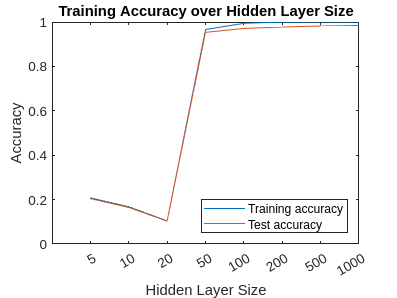
\includegraphics[width=\maxwidth{39.839438033115904em}]{figure_6.png}
\end{center}


\begin{matlabcode}
inputLayerSize = 784;
hiddenLayer1Size = 50;
outputLayerSize = 10;
[W1,b1,Wout,bout] = generate_weights(inputLayerSize,hiddenLayer1Size,outputLayerSize,0.1);

learningRate = [0.001,0.01,0.1,0.5,1,2,5,10];
numEpochs = 20;
batchsize = 100;

accuracy_history = zeros(length(learningRate), 1);
accuracy_test = zeros(length(learningRate), 1);

for p = 1:length(learningRate)
    lr = learningRate(p);
    for epoch = 1:numEpochs 
        for i = 1:size(X_train, 1)/batchsize
            % Use the permuted indices to get the current example and label
            X = X_train(1+batchsize*(i-1):batchsize*i,:);
            T = TTrain(1+batchsize*(i-1):batchsize*i,:);
            
            % Feedforward
            [A1,Z1,Aout,Zout] = forward_pass(X,W1,b1,Wout,bout);
            
            % Backpropagation
            [grad_W1, grad_b1, grad_Wout, grad_bout] = backward_pass(Zout, T, Z1, X, Wout, A1);
    
            % Update weights and biases
            [W1, b1, Wout, bout] = update_weights(lr,W1,b1,Wout,bout,grad_W1,grad_b1,grad_Wout,grad_bout);
        end
    end
    accuracy_history(p) = compute_accuracy(X_train, TTrain, W1, b1, Wout, bout);
    fprintf('Learning Rate %d: Accuracy: %0.5f\n', lr, accuracy_history(p));

    accuracy_test(p) = compute_accuracy(X_test, TTest, W1, b1, Wout, bout);
    fprintf('Learning rate %d: Test Accuracy: %0.5f\n', lr, accuracy_test(p));
end
\end{matlabcode}
\begin{matlaboutput}
Learning Rate 1.000000e-03: Accuracy: 0.98153
Learning rate 1.000000e-03: Test Accuracy: 0.96870
Learning Rate 1.000000e-02: Accuracy: 0.94405
Learning rate 1.000000e-02: Test Accuracy: 0.93680
Learning Rate 1.000000e-01: Accuracy: 0.09872
Learning rate 1.000000e-01: Test Accuracy: 0.09800
Learning Rate 5.000000e-01: Accuracy: 0.09872
Learning rate 5.000000e-01: Test Accuracy: 0.09800
Learning Rate 1: Accuracy: 0.09872
Learning rate 1: Test Accuracy: 0.09800
Learning Rate 2: Accuracy: 0.09872
Learning rate 2: Test Accuracy: 0.09800
Learning Rate 5: Accuracy: 0.09872
Learning rate 5: Test Accuracy: 0.09800
Learning Rate 10: Accuracy: 0.09872
Learning rate 10: Test Accuracy: 0.09800
\end{matlaboutput}


\begin{matlabcode}
figure;
plot(1:length(learningRate), accuracy_history);
hold on
plot(1:length(learningRate), accuracy_test);
title('Training Accuracy over LR');
legend('Training accuracy', 'Test accuracy','Location','northeast');
xlabel('Learning Rate');
ylabel('Accuracy');

% Specify the locations of the x-axis ticks
xticks(1:length(learningRate));

% Specify the labels of the x-axis ticks
xticklabels(learningRate);
\end{matlabcode}
\begin{center}
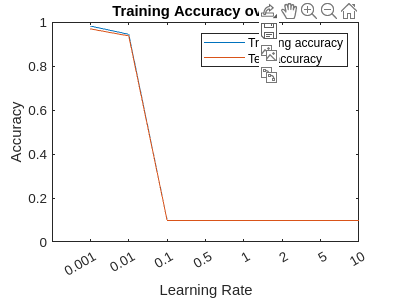
\includegraphics[width=\maxwidth{39.839438033115904em}]{figure_7.png}
\end{center}


\begin{matlabcode}
function ret = relu_func(z)
    ret = max(0,z);
end

function ret = relu_prime(z)
    ret = z>0;
end

function ret = softmax(z)
    ret = exp(z) ./ sum(exp(z),1);
end
    
function [W1, b1, Wout, bout] = generate_weights(input_size, layer1_size, output_size, scale)
    W1 = scale*(rand(layer1_size,input_size)-0.5);
    b1 = scale*(rand(layer1_size,1)-0.5);
    Wout = scale*(rand(output_size,layer1_size)-0.5);
    bout = scale*(rand(output_size,1)-0.5);
end

function [A1,Z1,Aout,Zout] = forward_pass(X,W1,b1,Wout,bout)
    % X has the nrows records with ncols features
    A1 = W1*X'+repmat(b1,1,size(X,1));
    Z1 = relu_func(A1);

    Aout = Wout*Z1+repmat(bout,1,size(X,1));
    Zout = softmax(Aout);
end

function [grad_W1, grad_b1, grad_Wout, grad_bout] = backward_pass(Zout, T, Z1, X, Wout, A1)
    % Error in output
    d_output = Zout - T';

    % Gradient for output weights and biases
    grad_Wout = d_output * Z1';
    grad_bout = sum(d_output, 2);

    % Error in first layer
    d_layer1 = (Wout' * d_output) .* relu_prime(A1);

    % Gradient for first layer weights and biases
    grad_W1 = d_layer1 * X;
    grad_b1 = sum(d_layer1, 2);
end

function [new_W1, new_b1, new_Wout, new_bout] = update_weights(lr,W1,b1,Wout,bout,grad_W1,grad_b1,grad_Wout,grad_bout)
    new_W1 = W1 - lr*grad_W1;
    new_b1 = b1 - lr*grad_b1;
    new_Wout = Wout - lr*grad_Wout;
    new_bout = bout - lr*grad_bout;
end

function accuracy = compute_accuracy(X, T, W1, b1, Wout, bout)
    % Feedforward
    [~, ~, ~, Zout] = forward_pass(X, W1, b1, Wout, bout);
    
    % Get the indices of the max values of the predicted and target labels
    [~, predicted_labels] = max(Zout);
    [~, true_labels] = max(T');
    
    % Compute accuracy
    accuracy = mean(predicted_labels == true_labels);
end

function pred = prediction(x,W1,b1,Wout,bout)
    [~, ~, ~, Zout] = forward_pass(x, W1, b1, Wout, bout);
    [~, predicted_labels] = max(Zout);
    pred = predicted_labels-1;
end
\end{matlabcode}

\end{document}
